\section{Introdução}
\label{sec:intro}

A adoção generalizada das tecnologias de Internet das Coisas (IoT), sistemas de monitoramento
industrial e aplicações financeiras em tempo real gerou um volume sem precedentes de dados
temporais, criando desafios críticos para as infraestruturas de armazenamento e análise.
Conforme projetado por~\cite{thierer2015iot}, o número de dispositivos IoT conectados vem
crescendo exponencialmente e deve continuar aumentando nos próximos anos, conforme ilustrado
na Figura~\ref{fig:iot_projection}.

\begin{figure}[ht]
  \centering
  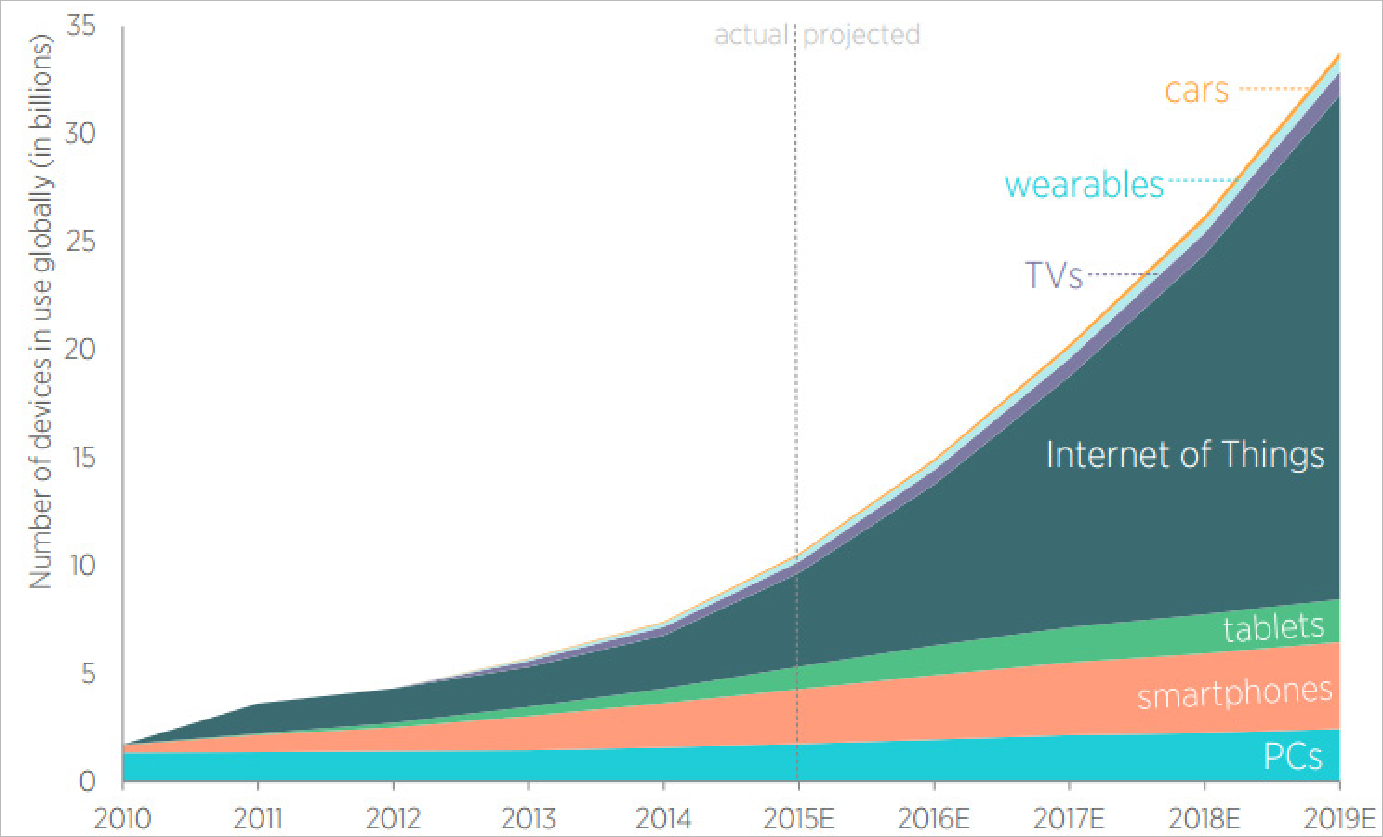
\includegraphics[width=\columnwidth]{figures/pt_br/projecao-iot}
  \caption{IoT: dispositivos em uso globalmente. Fonte:~\cite{thierer2015iot}.}
  \label{fig:iot_projection}
\end{figure}

Tal crescimento foi posteriormente reafirmado por~\cite{zikria2021nextgen}, que aponta que a Cisco prevê 500 bilhões de dispositivos conectados à IoT até 2030, enquanto a Telefonica estima que 90\% dos veículos estarão conectados e cada pessoa terá, em média, 15 dispositivos conectados nesse mesmo horizonte. A proliferação de aplicações de próxima geração, abrangendo saúde inteligente, cidades inteligentes, agricultura inteligente e IoT industrial, confirma que as projeções feitas em 2015 não apenas se concretizaram, mas continuam a se ampliar.

Como observado por~\cite{palma2016}, inúmeros setores passaram a depender da capacidade de
processar fluxos contínuos de dados. Entre eles: o setor financeiro, que utiliza essa
capacidade para analisar flutuações de ações e volumes de transações; os serviços de
transporte, que a empregam para monitorar viagens e migrações sazonais; a medicina, que a
utiliza para rastrear a disseminação de doenças; e a análise meteorológica, que aproveita
dados históricos para previsões mais precisas.

Esses fluxos de dados são sequências de eventos ou medições naturalmente ordenadas e indexadas
pelo tempo, frequentemente com precisão de milissegundos. Como observado por~\cite{Dunning2014},
o que costumava levar dez minutos para ser coletado em alguns sistemas muito ativos é agora
gerado a cada segundo. Essa explosão de dados sequenciais indexados por tempo expôs as
limitações fundamentais dos bancos de dados relacionais tradicionais quando confrontados com
padrões de acesso temporais, alta velocidade de ingestão e armazenamento histórico eficiente
de longo prazo.

Nesse cenário, os Bancos de Dados de Séries Temporais (BDSTs) emergiram como soluções
especializadas, arquitetadas desde a concepção para atender às demandas exclusivas dos dados
temporais~\citep{InfluxDataTimeSeries}. Como argumentado por~\cite{naqvi2017influxdb}, os
bancos de dados relacionais tradicionais sofrem de ineficiências de indexação e limitações de
memória ao lidar com grandes volumes de dados temporais, enquanto os BDSTs mantêm alto
desempenho por terem sido construídos com o tempo como preocupação central. Além da vazão
bruta, os BDSTs oferecem mecanismos especializados de compressão, co-localização de dados em
intervalos de tempo e políticas automáticas de retenção que reduzem os custos operacionais,
recursos indispensáveis para aplicações IoT onde medições contínuas de sensores demandam
escalabilidade e uso econômico de recursos~\citep{Dunning2014}.

O cenário dos BDSTs ampliou-se nos últimos anos, com sistemas adotando abordagens
arquiteturais distintas para o mesmo problema.
O \textit{Apache IoTDB}~\cite{wang2023iotdb}, desenvolvido na Universidade Tsinghua, foi
concebido especificamente para IoT industrial, utilizando um formato de arquivo colunar
personalizado (TsFile) e um protocolo binário RPC que possibilita taxas de ingestão
extremamente elevadas. O \textit{InfluxDB}, avaliado em quatro dos cinco estudos de desempenho revisados neste
trabalho~\citep{naqvi2017influxdb,shah2022performance,lima2024avaliando,wang2023iotdb}, usa
um motor de armazenamento Time-Structured Merge Tree (TSM) exposto via API HTTP com
protocolo de linha. O \textit{TimescaleDB} estende o PostgreSQL com capacidades de séries
temporais~\citep{Ramakrishnan2003}, oferecendo compatibilidade com SQL e o ecossistema
relacional completo como contrapartida a uma menor vazão bruta de escrita. Cada abordagem
possui pontos fortes e fracos distintos que não são aparentes apenas a partir de descrições
e exigem medições controladas sob cargas de trabalho IoT realistas.

O campo de benchmarking de BDSTs, no entanto, sofre de uma lacuna metodológica crítica: a
falta de reprodutibilidade. Uma análise dos estudos comparativos recentes revela que a maioria
dos benchmarks publicados não fornece scripts, configurações ou versões exatas de software
suficientes para permitir replicação independente~\citep{pereira2023mulletbench,shah2022performance,naqvi2017influxdb}.
Sem metodologia reprodutível, os resultados não podem ser validados de forma independente,
são difíceis de comparar entre estudos e os experimentos não podem ser adaptados a novos
hardwares ou versões de software. Este trabalho aborda diretamente essa lacuna tornando a
infraestrutura completa de benchmark (todos os scripts de orquestração, definições de
contêineres, ambiente de construção e clientes de benchmark parametrizados)
publicamente disponível junto com os resultados.

Este artigo apresenta uma comparação controlada e reprodutível do Apache IoTDB, InfluxDB~2.7
e TimescaleDB em nove padrões de carga de trabalho representativos de implantações IoT e
três escalas de volume de dados. Os bancos de dados foram selecionados com base em sua
proeminência na literatura comparativa recente: InfluxDB como o padrão de referência
estabelecido, Apache IoTDB como o líder emergente nos dois estudos mais recentes~\citep{pereira2023mulletbench,wang2023iotdb},
e TimescaleDB como a alternativa baseada em SQL que oferece ampla compatibilidade com
ecossistemas. A metodologia de benchmark foi projetada para isolar propriedades arquiteturais
de artefatos de medição, incluindo uma comparação explícita entre execuções originais com
recursos compartilhados e reexecuções isoladas e devidamente ajustadas, para validar quais
descobertas refletem o comportamento genuíno de cada banco de dados.

Os objetivos específicos deste trabalho são:
\begin{itemize}
  \item Medir o desempenho de escrita e leitura de três BDSTs em cargas de trabalho
    representativas de implantações IoT reais;
  \item Analisar como as características de desempenho escalonam com o volume de dados
    em três escalas com variação de cem vezes no tamanho dos dados;
  \item Identificar os mecanismos arquiteturais que explicam as diferenças de desempenho
    observadas;
  \item Quantificar o impacto das escolhas metodológicas do benchmark nos resultados
    reportados; e
  \item Fornecer uma infraestrutura de benchmark reprodutível que permita a pesquisadores
    futuros validar e estender de forma independente estes resultados.
\end{itemize}

O restante deste artigo está organizado da seguinte forma.
A Seção~\ref{sec:theoretical} apresenta a fundamentação teórica cobrindo bancos de dados,
bancos de dados de séries temporais e conceitos de benchmarking.
A Seção~\ref{sec:related} revisa estudos comparativos relacionados e identifica as lacunas
que motivam este trabalho.
A Seção~\ref{sec:methodology} descreve a metodologia de benchmark, o projeto das cargas de
trabalho e a infraestrutura reprodutível.
A Seção~\ref{sec:experiments} apresenta e analisa os resultados experimentais.
A Seção~\ref{sec:conclusion} conclui o artigo com uma comparação final e direções para
trabalhos futuros.
